% # Testando LaTeX

\chapter{Removendo <> da URL}

\def\LinkTest{https://www.example.com/page.html}

\begin{enumerate}
  \item LinkToURL: \LinkToURL{\LinkTest}{Exemplo}
  \item URL: \url{\LinkTest}
  \item \cite{test1}
  \item \cite{test2}
  \item \cite{test3}
\end{enumerate}

% \chapter{Teste RGB}

% Teste pra saber de que forma que o filtro de cor cinza no vscode tá afetando a visualização das minhas imagens.

% \begin{MyCenteredFigure} \caption{Teste de RGB}
%   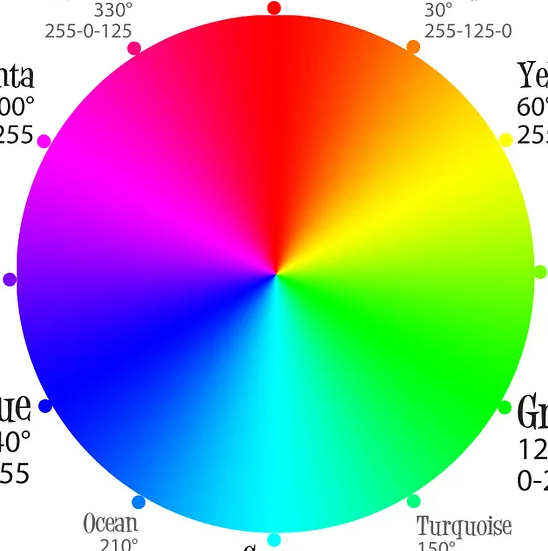
\includegraphics[width=0.5\textwidth]{files/img/unused/teste RGB.png}
% \end{MyCenteredFigure}

% \chapter{Embedding}

ATACHING

% \attachfile{files/codigos/ATTACH.txt}

% test \textattachfile[color=1 0 0]{files/codigos/ATTACH.txt}{Texto 1}

% test \textattachfile[color=0 1 1]{files/codigos/ATTACH.txt}{Texto 2}

% \textattachfile[]{files/codigos/CodigoFonteLaTeX.rar.RemovaEstaPartaParaAcessarOCodigo}{Texto 3}

% EMBEDING

% \embedfile[desc={DECRICAO}]{files/codigos/EMBED.txt}

% \embedfile[desc={DECRICAO2}]{files/codigos/CódigoFonte.rar}

% \embedfile[desc={DECRICAO3}]{files/codigos/CódigoFonte.rar.RemovaEstaPartaParaAcessarOCódigo}

% \embeddedfile{alias}{files/codigos/EMBED2.txt}

% \openfilelink{files/codigos/EMBED2.txt}{Clique aqui para abrir o arquivo}


% \chapter{Easter Egg}

% \begin{MyCenteredFigure}
%   \caption{Teste de Easter Egg}
%   
\includegraphics[width=0.5\textwidth]{files/img/unused/teste}

%   \adjustbox{trim={.25\width} {.25\height} {.25\width} {.25\height},clip}{
\includegraphics[width=0.5\textwidth]{files/img/unused/teste}}
% \end{MyCenteredFigure}

% \chapter{Build}

1

ABCDEFGHIJKLMNOPQRSTUVWXYZ

2
